\section{Импульс}

\subsection{Определение импульса}
\textbf{Импульс материальной точки} --- векторная физическая величина, являющаяся мерой механического движения и равная произведению массы точки на её скорость:
\[
    \vec{p} = m\vec{v}
\]

Согласно второму закону Ньютона в дифференциальной форме, скорость изменения импульса тела равна действующей на него силе:
\[
    \frac{d\vec{p}}{dt} = \vec{F}
\]
Эта запись является более общей, чем $\vec{F} = m\vec{a}$, так как применима и в случаях переменной массы.

\subsection{Центр масс системы}
\textbf{Центром масс} системы материальных точек называется точка $C$, радиус-вектор которой определяется как:
\[
    \vec{r}_{cm} = \frac{\sum m_i \vec{r}_i}{\sum m_i} = \frac{1}{M} \sum m_i \vec{r}_i
\]
Движение абсолютно твердого тела можно полностью описать как движение его центра масс и вращение вокруг него:

\begin{center}
\begin{tblr}{
  colspec = {X[1.2,c]X[2,c]},
  vlines,
  hlines,
  row{1} = {font=\bfseries,mode=text},
  row{odd} = {bg=gray!10},
  cells = {mode=math,c,m},
  rowsep = 6pt
}
\text{Центр масс системы} & \text{Формулы и свойства} \\
\text{Скорость системы} & \vec{V}_c = \dfrac{\diff\vec{R}}{\diff t} = \dfrac{\sum m_i\vec{v}_i}{\sum m_i} \\
\text{Импульс системы} & \vec{P}_c = M\vec{V}_c = \sum m_i\vec{v}_i
\end{tblr}
\end{center}

\subsection{Закон сохранения импульса}
В \textbf{изолированной системе} не действуют внешн. силы или их сумма нулевая:
\[\sum \vec{F} = 0\]

Для системы материальных точек:
\[
    \frac{d\vec{P}}{dt} = \sum \vec{F}
\]
Если система изолированная, то $\frac{d\vec{P}}{dt} = 0$, следовательно:
\[\boxed{
    \vec{P} = \sum m_i \vec{v}_i = \text{const}
}\]
То есть центр масс замкнутой системы движется равномерно и прямолинейно или покоится.

\subsection{Уравнение Мещерского}

\subsubsection{Формулировка}
Уравнение описывает движение тела с переменной массой (например, ракеты):

\begin{center}
\begin{tblr}{
  colspec = {X[1.2,l]X[1,c]},
  vlines,
  hlines,
  row{1} = {font=\bfseries,mode=text},
  row{odd} = {bg=gray!10},
  cells = {c,m},
  rowsep = 8pt,
  width = \textwidth
}
Уравнение Мещерского & Схема процессов массы \\
\parbox{0.5\textwidth}{
\centering
\large
$m(t)\dfrac{\diff\vec{v}}{\diff t}=\vec{u_1}\dfrac{\diff m_1}{\diff t}-\vec{u_2}\dfrac{\diff m_2}{\diff t}+\vec{F}$ \\
\normalsize
\begin{align*}
m(t) &- \text{мгновенная масса} \\
\vec{u_1} &= \vec{v}_1 - \vec{v} \quad \text{(отн. присоединение)} \\
\vec{u_2} &= \vec{v}_2 - \vec{v} \quad \text{(отн. выброс)} \\
\vec{F} &- \text{внешние силы}
\end{align*}
}
&
\begin{minipage}[c]{\linewidth}
\centering
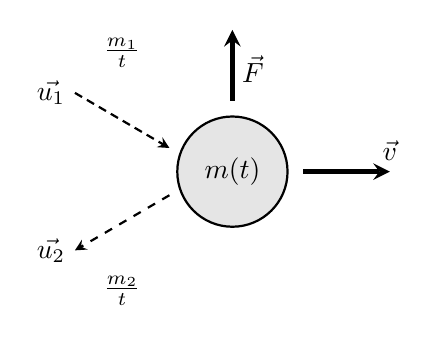
\begin{tikzpicture}[scale=1.0, >=stealth]
    % Основное тело с штриховкой для ч/б печати
    \draw[fill=black!10, thick] (0,0) circle (0.7);
    \node at (0,0) {$m(t)$};
    
    % Стрелка движения тела (сплошная толстая)
    \draw[->, ultra thick] (0.9,0) -- (2.0,0) node[above] {$\vec{v}$};
    
    % Присоединяемая масса (штрих-пунктир)
    \draw[->, thick, densely dashed] (-2.0,1.0) -- (-0.8,0.3);
    \node[left] at (-2.0,1.0) {$\vec{u_1}$};
    \node[above] at (-1.4,1.2) {$\frac{\diff m_1}{\diff t}$};
    
    % Отделяемая масса (пунктир)
    \draw[->, thick, dashed] (-0.8,-0.3) -- (-2.0,-1.0);
    \node[left] at (-2.0,-1.0) {$\vec{u_2}$};
    \node[below] at (-1.4,-1.2) {$\frac{\diff m_2}{\diff t}$};
    
    % Внешние силы (двойная линия)
    \draw[->, ultra thick] (0,0.9) -- (0,1.8);
    \node[right] at (0,1.3) {$\vec{F}$};
\end{tikzpicture}
\end{minipage}
\\
\end{tblr}
\end{center}

\subsubsection{Вывод}

Рассмотрим тело переменной массы $m(t)$, движущееся со скоростью $\vec{v}(t)$. Пусть за время $dt$ к телу присоединяется масса $dm_1 > 0$ со скоростью $\vec{v}_1$ относительно Земли, а отделяется масса $dm_2 > 0$ со скоростью $\vec{v}_2$ относительно Земли.

Введем относительные скорости:
\begin{align*}
\vec{u}_1 &= \vec{v}_1 - \vec{v} \text{ --- относительная скорость присоединяемой массы}, \\
\vec{u}_2 &= \vec{v}_2 - \vec{v} \text{ --- относительная скорость отделяемой массы}.
\end{align*}

Тогда:
\[
\vec{v}_1 = \vec{v} + \vec{u}_1, \qquad \vec{v}_2 = \vec{v} + \vec{u}_2.
\]

Изменение массы тела за время $dt$:
\[
dm = dm_1 - dm_2
\]

Импульс системы в момент времени $t$:
\[
\vec{p}(t) = m\vec{v}.
\]

Импульс системы в момент времени $t+dt$:
\begin{align*}
\vec{p}(t+dt) &= (m + dm)(\vec{v} + d\vec{v}) + (-dm_1)\vec{v}_1 + (+dm_2)\vec{v}_2 \\
&= (m + dm)(\vec{v} + d\vec{v}) - dm_1(\vec{v} + \vec{u}_1) + dm_2(\vec{v} + \vec{u}_2).
\end{align*}

Изменение импульса под действием внешней силы $\vec{F}$:
\[
\vec{F}\, dt = \vec{p}(t+dt) - \vec{p}(t).
\]

Подставляем выражения для импульсов:
\begin{align*}
\vec{F}\, dt &= \big[(m + dm)(\vec{v} + d\vec{v}) - dm_1(\vec{v} + \vec{u}_1) + dm_2(\vec{v} + \vec{u}_2)\big] - m\vec{v} \\
&= m\vec{v} + m d\vec{v} + \vec{v}\, dm + dm\, d\vec{v} - \vec{v}\, dm_1 - \vec{u}_1 dm_1 + \vec{v}\, dm_2 + \vec{u}_2 dm_2 - m\vec{v} \\
&= m d\vec{v} + \vec{v}(dm - dm_1 + dm_2) + \vec{u}_2 dm_2 - \vec{u}_1 dm_1 + dm\, d\vec{v}.
\end{align*}

Учитывая, что $dm = dm_1 - dm_2$, получаем $dm - dm_1 + dm_2 = 0$. Пренебрегая членом второго порядка $dm\, d\vec{v}$, имеем:
\[
\vec{F}\, dt = m d\vec{v} + \vec{u}_2 dm_2 - \vec{u}_1 dm_1.
\]

Разделим на $dt$:
\[
\vec{F} = m \frac{d\vec{v}}{dt} + \vec{u}_2 \frac{dm_2}{dt} - \vec{u}_1 \frac{dm_1}{dt}.
\]

Перегруппировав слагаемые, получаем:
\[\boxed{
m(t) \frac{d\vec{v}}{dt} = \vec{u}_1 \frac{dm_1}{dt} - \vec{u}_2 \frac{dm_2}{dt} + \vec{F}
}\]